\begin{problem}[问题4.3]如右图所示, L型等截面管的A
\vspace{-2em}

\begin{multicols}{2}
~

B和BC两段各长为L, 内充满不可压缩理想流体,
初始时刻C端封闭. 某时刻C端突然打开, 求:
\begin{enumerate}
\item 此刻管内流体的加速度大小.
\item 沿管的压强分布.
\end{enumerate}
\textbf{思考:}如果竖直管道截面积是水平管道的两倍, 情况又如何变化.
\begin{center}
\usetikzlibrary{%
    decorations.pathreplacing,%
    decorations.pathmorphing,arrows
}
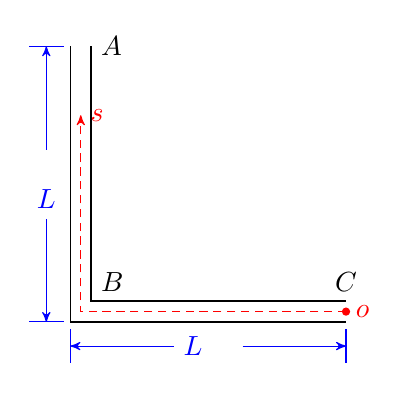
\begin{tikzpicture}[scale=1.75]
\draw[semithick](0,2)--(0,0)--(2,0);
\draw[semithick](0.15,2)node[right]{$A$}--(0.15,0.15)node[above right]{$B$}--(2,0.15) node[above]{$C$};
\fill[red] (2,0.075) node[right]{$o$}circle(0.03);
\draw[densely dashed,red,->,>=stealth'] (2,0.075)--(0.075,0.075)--(0.075,1.5) node[right]{$s$};
\draw[blue](-0.05,2)--(-0.3,2) (-0.05,0)--(-0.3,0) (0,-0.05)--(0,-0.3) (2,-0.05)--(2,-0.3);

\draw[blue,<-,>=stealth'] (-0.175,0)--(-0.175,0.75) node[above]{$L$}; 
\draw[blue,->,>=stealth'] (-0.175,1.25)--(-0.175,2); 

\draw[blue,<-,>=stealth'] (0,-0.175)--(0.75,-0.175) node[right]{$L$}; 
\draw[blue,->,>=stealth'] (1.25,-0.175)--(2,-0.175); 
\end{tikzpicture}

\end{center}
\end{multicols}
\end{problem}

\begin{solution}
\textbf{解:}
如图中所示, 以$C$为原点,建立沿L型等截面管的自然坐标系$s$. 因为L型管AB段(或BC段)等截面, 因此液体在AB段(或BC段)任意点的速度和加速度都相等. 即$\frac{\partial v}{\partial s} = 0$. 故速度势
\[
\varphi(s,t) =\begin{dcases}
 v_{AB}(t)s & s \leq L \\
v_{AB}(t)L + v_{BC}(t)(s-L) & s > L
\end{dcases}
\]
对$t=0$时刻的$A,C$及任意一点$s$应用Bernoulli方程
\begin{equation}
\frac{\partial\varphi_A}{\partial t} + \frac{1}{2}v_A^2 + \frac{p_A}{\rho} + gz_A = \frac{\partial\varphi_C}{\partial t} + \frac{1}{2}v_C^2 + \frac{p_C}{\rho} + gz_C =
\frac{\partial\varphi_s}{\partial t} + \frac{1}{2}v_s^2 + \frac{p_s}{\rho} + gz_s
\end{equation}
$t=0$时刻的$A,C$及任意一点$s$的速度$v_A = v_C = v_s=0$. 故上式可化为
\[
L\frac{\partial v_A}{\partial t} + L\frac{\partial v_C}{\partial t} + gL = 0
\]

\[
\begin{dcases}
 s\frac{\partial v_s}{\partial t} + \frac{p_s}{\rho} = \frac{p_C}{\rho} = \frac{p_C}{\rho}=\frac{p_0}{\rho} & s \leq L \\
 (s-L)\frac{\partial v_s}{\partial t} + L\frac{\partial v_C}{\partial t} + \frac{p_s}{\rho} + g(s-L) =  \frac{p_C}{\rho} = \frac{p_0}{\rho} & s > L
\end{dcases}
\]
由于$dv_A/dt=\partial v_A/\partial t + v_A \partial v_A/\partial s = \partial v_A/\partial t = a_A$.同理$\partial v_C/\partial t = a_C$ 因此有
\begin{equation}\label{a}
L\frac{d v_A}{d t} + L\frac{d v_C}{d t} + gL = 0 \Longrightarrow a_A + a_C = -g
\end{equation}
\begin{equation}\label{p}
p_s = \begin{dcases}
p_0 - s\rho a_C & s \leq L \\
p_0 - \rho[(s-L)a_A + La_C + g(s-L)]& s > L
\end{dcases}
\end{equation}
下面分别考虑以下两种情况
\begin{itemize}
\item \textbf{竖直管道截面积 = \textcolor{white}{2}水平管道的面积:} $a_C = a_A$

将$a_C = a_A$代入式(\ref{a})得液体加速度
\[
a = a_C = a_A = - \frac{1}{2}g
\]
其中负号表示液体加速度与自然坐标系$s$的正方向相反. 将加速度代入式(\ref{p})得
\[
p_s = 
\begin{dcases}
p_0 + \frac{1}{2}\rho gs & s \leq L \\
p_0 + \frac{1}{2}\rho g(2L-s) & s > L
\end{dcases}
\]

\item \textbf{竖直管道截面积 = 2水平管道的面积:} $a_C = 2a_A$


将$a_C = 2a_A$代入式(\ref{a})得液体加速度
\[
a_C =  - \frac{2}{3}g,{~~} a_A = - \frac{1}{3}g
\]
其中负号表示液体加速度与自然坐标系$s$的正方向相反. 将加速度代入式(\ref{p})得
\[
p_s = \begin{dcases}
p_0 + \frac{2}{3}\rho gs & s \leq L \\
p_0 + \frac{2}{3}\rho g(2L-s) & s > L
\end{dcases}
\]

\end{itemize}



\end{solution} 
